\chapter{State of the art}
\label{cha:state-of-the-art}

%% W3Tech chart of server-side language share
\begin{figure}[p]
    \centering
    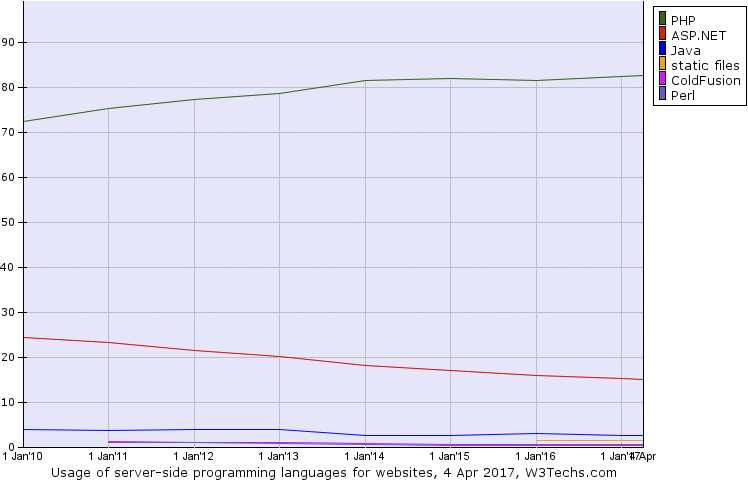
\includegraphics[width=0.9\textwidth]{server-side-languages.png}
    \caption{A graphic showing the global share of \textbf{server-side programming languages} from January 2010 to April 2017. \texttt{PHP} remains the dominant language with a share growing from \textbf{72.5\%} to \textbf{82.6\%}.}
    \label{fig:server-side-languages}
\end{figure}
%

The roots of the most well-known modern Content Management Systems (\emph{CMS}) date back to the early 2000s, when PHP was (and \emph{still is}) the dominant factor in terms of server-side programming languages (See Fig. \ref{fig:server-side-languages}). %% Please check, if reference is accurate enough

While the \emph{typical} CMS was starting out as mostly just a ``dynamic online tool'', it also shows that with seamlessly integrating new features gained through the development of its underlying programming languages, as well as steadily adding new functionalities (mostly requested by the community), a transition towards a fully-manageable and customizeable, semi-automatic web application was possible \cite[17]{dhillon2016}.

However, this progression also caused a few drawbacks, especially when it comes down to comparing the amount of workload needed before being able to actually create content for the World Wide Web. Due to the fact, that most CMS contain their own sort of plugin management

on the one hand it shows the ease of bringing new content online, whereas on the other hand

\section{Jekyll}
\label{sec:jekyll}

As already explained, Jekyll was created out of the need for avoiding to service the blogging engine before writing and publishing content. Since it is deeply integrated into \emph{GitHub}, it is considered as the probably most-popular static site generator.

\subsection{History}
\label{sec:jekyll-history}
\emph{Tom Preston-Werner}, co-founder of GitHub\footnote{\url{https://github.com} -- GitHub Inc.}, announced it in October 2008 in one of his blog posts \cite{PrestonWerner2008jekyll}. Already in December 2008, it was introduced as build engine for the then newly featured GitHub Pages service, allowing owners of repositories to publish a static website by just pushing to a certain \emph{master} or \emph{gh-pages} branch \cite{PrestonWerner2008githubpages}, which is still available for free to this day.

All of this happened just 6 (respectively 8) months after GitHub was launched \cite{PrestonWerner2008githublaunch} and is now even being used by technology-leading companies to showcase their Open-Source efforts\footnote{\url{https://github.com/showcases/github-pages-examples} -- GitHub Pages examples.}.

\subsection{Technology}
\label{sec:jekyll-technology}
Jekyll was entirely written in \emph{Ruby}, as Tom Preston-Werner rather saw himself as a software developer in the first place, than as a content author \cite{PrestonWerner2008jekyll}. Until now, the repository for Jekyll still consists mainly of Ruby code at a share of roughly 77.5\%.

\subsubsection{Advantages}
One of the main advantages is the modular structure of its code base. By inheriting different Ruby classes, it is quite easy to extend and add features to fit the developer's needs. Due to its wide-spread usage initiated through the GitHub universe, Jekyll also has an accordingly huge user base and is therefore well documented \cite[26]{dhillon2016}.

Furthermore, its website\footnote{\url{http://jekyllrb.com} -- Jekyll website.}, which mainly acts as starting basis for documentation, is not only available as open-sourced git repository, it is also built using \texttt{Jekyll} to prove its universality.

Starting from scratch, the command \texttt{jekyll new my\_project} installs a blog environment for starters in the \texttt{./my\_project} folder. The basic install consists of an elementar blog post structure, \emph{Sass} source files, and a few template files written for Shopify's \emph{Liquid}\footnote{\url{https://help.shopify.com/themes/liquid} -- Shopify's Liquid template engine.} engine.\\
Using this starting environment, the unexperienced developer quickly gets a sufficient overview of what is generally possible using Jekyll, whereas the content author is able to fully concentrate himself on writing content, as the used \emph{Markdown} markup language requires little to no prior syntax knowledge. Furthermore, Jekyll already ships with a built-in webserver for quickly reviewing the rendered static output.

\subsubsection{Disadvantages}
As powerful as Ruby might be designed, many unskilled developers are facing difficulties right from the beginning, as most of them experience a steep learning curve. Nearly every single bit of customizing Jekyll requires Ruby knowledge, especially if it is desired to move along the ``predefined'' way and not including third-party extensions like \emph{Node.js} tools or else.

Additionally, its template language, Liquid, offers customization on a very high level, so it might happen to confuse business logic\footnote{How Jekyll processes data into programmatically readable structures.} with template logic\footnote{How Liquid transforms these structures into browser-readable HTML.}. To make things worse, different template constructions might also evolve over time and therefore causing a parallel coding universe when trying to surpass difficulties in the business logic.

%% bring some difficulties concerning ruby versions
%% ruby gems

